\documentclass[../main.tex]{subfiles}

\begin{document}

\subsection{Problem decomposition\label{subsection:problem-decomposition}}

I have decomposed the problem of visualization as follows:
\begin{center}
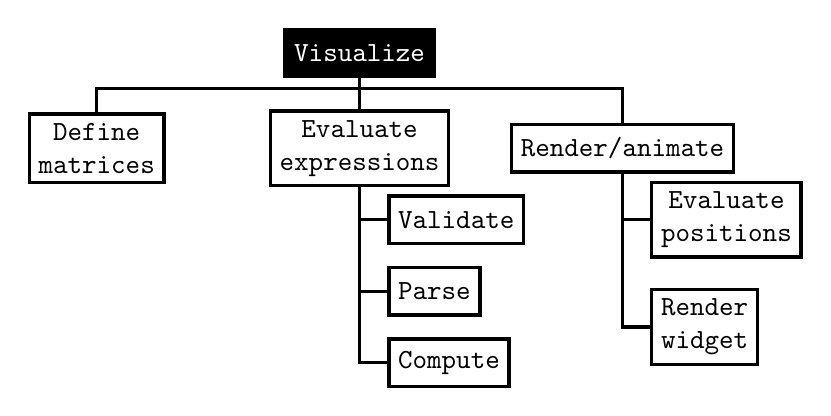
\begin{tikzpicture}[
	every node/.style={rectangle, minimum size=6mm, draw=black, font=\ttfamily, align=center, very thick},
	every path/.style={very thick},
	root/.style={rectangle, text=white, fill=black},
	module/.style={text=black, grow=down, anchor=west, edge from parent path={\tikzparentnode.south |- \tikzchildnode.west}},
	vertical/.style={grow=down, xshift=1em, anchor=west, edge from parent path={(\tikzparentnode.south) |- (\tikzchildnode.west)}, level distance={#1*6ex}},
	level 1/.style={sibling distance=9.5em},
]
\node [root] {Visualize}
	child [grow=down, level distance=5ex, shape=coordinate] {
		child [grow=down, level distance=-2ex] [edge from parent path={(\tikzparentnode.south) -| (\tikzchildnode.north)}]
		child {node {Define\\matrices}}
		child {node {Evaluate\\expressions}
			child [vertical=1] {node [module] {Validate}}
			child [vertical=2] {node [module] {Parse}}
			child [vertical=3] {node [module] {Compute}}
		}
		child {node {Render\slash animate}
			child [vertical=1] {node [module] {Evaluate\\positions}}
			child [vertical=2.5] {node [module] {Render\\widget}}
		}
	};
\end{tikzpicture}
\end{center}
Defining matrices is key to visualization because we need to have matrices to actually visualize. This is a key part of the app, and the user will be able to define multiple separate matrices numerically and visually using the GUI.

Evaluating expressions is another key part of the app and can be further broken down into validating, parsing, and computing the value. Validating an expression simply consists of checking that it adheres to a set of syntax rules for matrix expressions, and that it only contains matrices which have already been defined. Parsing consists of breaking an expression down into tokens, which are then much easier to evaluate. Computing the expression with these tokens is then just a series of simple operations, which will produce a final matrix at the end.

Rendering and animating will likely be the largest part in reality, but I've only decomposed it into simple blocks here. Evaluating positions involves evaluating the matrix expression that the user has input and using the columns of the resultant matrix to find the new positions of the basis vectors, and then extrapolating this for the rest of the plane. Rendering onto the widget is likely to be quite complicated and framework-dependent, so I've abstracted away the details for brevity here. Rendering will involve using the previously calculated values to render grid lines and vectors. Animating will probably be a \texttt{for} loop which just renders slightly different matrices onto the widget and sleeps momentarily between frames.

I have deliberately broken this problem down into parts that can be easily translated into modules in my eventual coded solution. This is simply to ease the design and development process, since now I already know my basic project structure. This problem could've been broken down into the parts that the user will directly interact with, but that would be less useful to me when actually starting development, since I would then have to decompose the problem differently to write the actual code.

\end{document}
